\documentclass[a4paper,12pt]{article}
\usepackage{fancyhdr}
\usepackage{lastpage}
\usepackage{geometry}
\usepackage{listings}
\usepackage{datetime}
\usepackage{xeCJK}
\usepackage{hyperref}
\usepackage{amsmath}
\usepackage{graphicx}
\usepackage{float} % 加入 float 宏包以使用 [H]
\usepackage{longtable}

\geometry{left=2.5cm, right=2.5cm, top=2.5cm, bottom=2.5cm}
\pagestyle{fancy}
\setCJKmainfont{Noto Sans TC}
% 英文字體 consolas
\setmonofont{Consolas}
% 設定內文文字大小
\renewcommand{\normalsize}{\fontsize{12pt}{\baselineskip}\selectfont}

% 設定頁首
\fancyhf{}
\fancyhead[L]{Volume Rendering and Gradient Visualization(HW2)}
\fancyhead[R]{\today}
\fancyfoot[C]{\thepage/\pageref{LastPage}}

\title{Volume Rendering and Gradient Visualization(HW2)}
\author{01057033洪銘均}
\date{\today}

\begin{document}
\maketitle
\tableofcontents
\newpage

\section{程式概述}
該程式使用imgui搭配資料處理與統計的方式,在預處理時利用CDF均衡化統計資料不平衡,再計算梯度後利用imgui做梯度與統計數據的視覺化



\section{運行結果}

\begin{figure}[h]
    \centering
    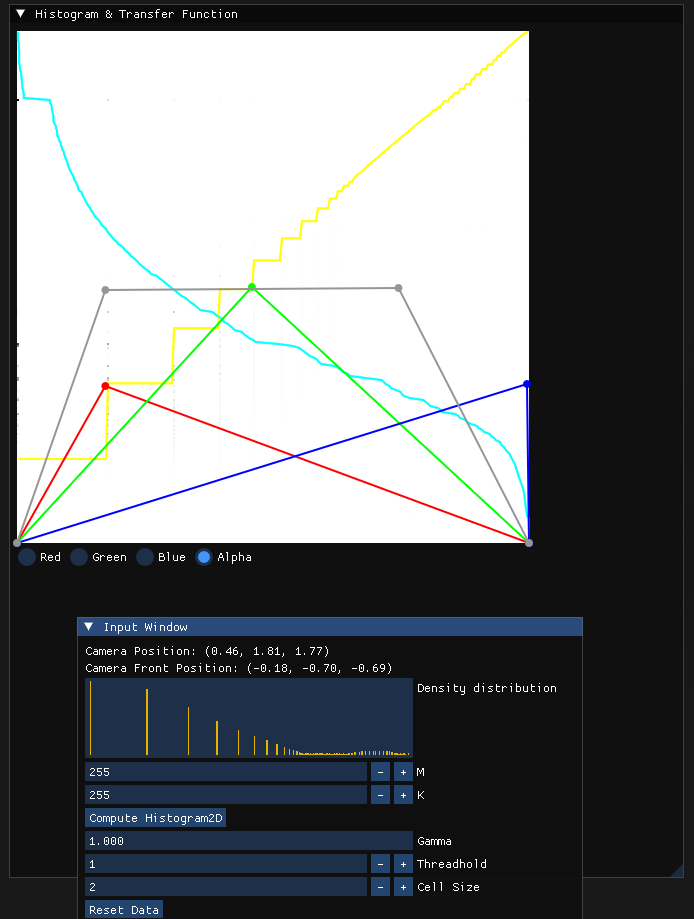
\includegraphics[width=0.8\textwidth]{img/img2.png}
\end{figure}
圖中縱軸為梯度值、橫軸為密度值,黃色為密度值累積、青色為梯度值累積,可以看到利用CDF映射後成功讓資料分散化,極值也利用CDF讓其值有所下降並且較為平滑。

\section{心得}
這次作業成功了解到利CDF映射作為equalizer,並成功讓極值下降,使整體趨勢較為平滑化,一開始使用Gamma校正、移除域值、以及刪除空缺的硬度值的方式,但效果校為不佳,且極值過大的問題依舊存在,使用CDF後才較為正常。
\end{document}

% xelatex  --max-print-line=10000 -synctex=1 -interaction=nonstopmode -file-line-error -recorder .\codebook.tex 
